\documentclass[tikz,border=8pt]{standalone}
\usepackage{amsmath}
\usepackage[T1]{fontenc}
\usepackage{tikz}
\usetikzlibrary{positioning,arrows.meta,backgrounds,fit,calc}

\begin{document}

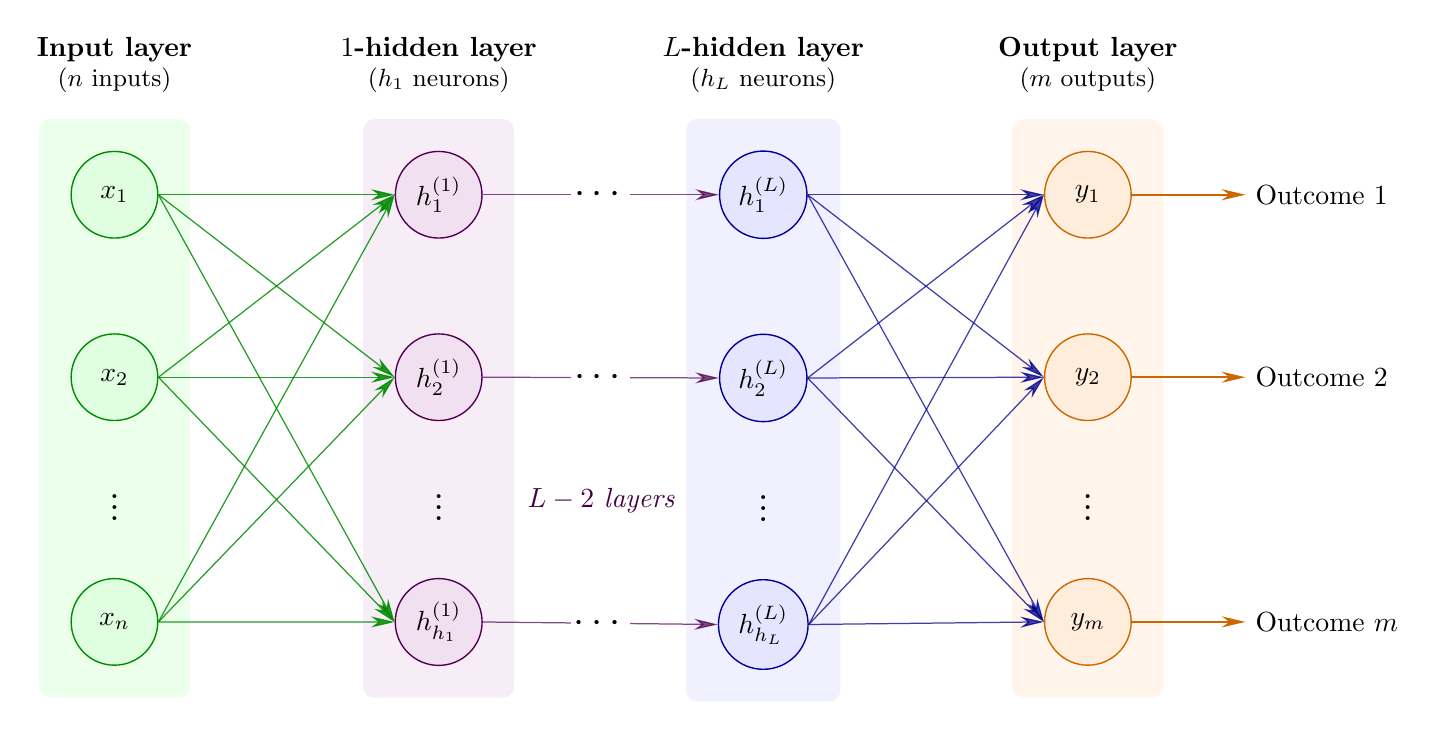
\begin{tikzpicture}[
    >={Stealth[length=3mm, width=1.4mm]},
    font=\normalsize,
    neuron/.style   = {circle, draw, minimum size=11mm, line width=0.5pt},
    input/.style    = {neuron, draw=green!55!black,  fill=green!12},
    hiddenA/.style  = {neuron, draw=violet!65!black, fill=violet!12},
    hiddenB/.style  = {neuron, draw=blue!60!black,   fill=blue!10},
    output/.style   = {neuron, draw=orange!80!black, fill=orange!14},
    egreen/.style   = {->, green!55!black,  opacity=0.85, line width=0.45pt},
    eviolet/.style  = {->, violet!60!black, opacity=0.70, line width=0.45pt},
    eblue/.style    = {->, blue!55!black,   opacity=0.75, line width=0.45pt},
    eorange/.style  = {->, orange!80!black, line width=0.7pt},
    node distance = 12mm and 30mm,
    dots/.style   = {font=\Large}
]

% INPUT LAYER
\node[input] (x1) {$x_1$};
\node[input, below=of x1] (x2) {$x_2$};
\node[dots, below=6mm of x2] (xd) {$\vdots$};
\node[input, below=6mm of xd] (xn) {$x_n$};

% HIDDEN LAYER 1
\node[hiddenA, right=of x1] (a1) {$h^{(1)}_1$};
\node[hiddenA, below=of a1] (a2) {$h^{(1)}_2$};
\node[dots, below=6mm of a2] (ad) {$\vdots$};
\node[hiddenA, below=6mm of ad] (an) {$h^{(1)}_{h_1}$};

% HIDDEN LAYER L
\node[hiddenB, right=of a1] (b1) {$h^{(L)}_1$};
\node[hiddenB, below=of b1] (b2) {$h^{(L)}_2$};
\node[dots, below=6mm of b2] (bd) {$\vdots$};
\node[hiddenB, below=6mm of bd] (bn) {$h^{(L)}_{h_L}$};

% OUTPUT LAYER
\node[output, right=of b1] (y1) {$y_1$};
\node[output, below=of y1] (y2) {$y_2$};
\node[dots, below=6mm of y2] (yd) {$\vdots$};
\node[output, below=6mm of yd] (ym) {$y_m$};

% EDGES: input -> hidden1  (salida en .east, llegada radial al centro)
\foreach \i in {x1,x2,xn}{
  \foreach \j in {a1,a2,an}{ \draw[egreen] (\i.east) -- (\j.west); }
}

% EDGES: hidden1 -> hiddenL  (horizontales puras .east -> .west)
\foreach \i/\j in {a1/b1, a2/b2, an/bn}{ \draw[eviolet] (\i.east) -- (\j.west); }

% EDGES: hiddenL -> output  (salida en .east, llegada radial)
\foreach \i in {b1,b2,bn}{
  \foreach \j in {y1,y2,ym}{ \draw[eblue] (\i.east) -- (\j.west); }
}

% output arrows
\foreach \k/\lbl in {y1/Outcome 1, y2/Outcome 2, ym/Outcome $m$}{
  \draw[eorange] (\k) -- ++(2.0cm,0) node[right, black]{\lbl};
}

% \cdots centrados sobre las flechas horizontales
\node[dots, fill=white, inner sep=1pt] at ($(a1.east)!0.5!(b1.west)$) {$\cdots$};
\node[dots, fill=white, inner sep=1pt] at ($(a2.east)!0.5!(b2.west)$) {$\cdots$};
\node[dots, fill=white, inner sep=1pt] at ($(an.east)!0.5!(bn.west)$) {$\cdots$};

% Etiqueta "L layers" en la fila de los vdots
\node[font=\itshape, text=violet!55!black] at ($(ad)!0.5!(bd)$) {$L-2$ layers};

% BACKGROUND PANELS
\begin{scope}[on background layer]
  \node[fill=green!8,  rounded corners, fit=(x1)(xn), inner sep=4mm] (pIn)  {};
  \node[fill=violet!7, rounded corners, fit=(a1)(an), inner sep=4mm] (pA)   {};
  \node[fill=blue!6,   rounded corners, fit=(b1)(bn), inner sep=4mm] (pB)   {};
  \node[fill=orange!8, rounded corners, fit=(y1)(ym), inner sep=4mm] (pOut) {};
\end{scope}

\node[align=center, above=2mm of pIn,  font=\bfseries]
    {Input layer\\[-1pt]\normalfont\small ($n$ inputs)};
\node[align=center, above=2mm of pA,   font=\bfseries]
    {$1$-hidden layer\\[-1pt]\normalfont\small ($h_1$ neurons)};
\node[align=center, above=2mm of pB,   font=\bfseries]
    {$L$-hidden layer\\[-1pt]\normalfont\small ($h_L$ neurons)};
\node[align=center, above=2mm of pOut, font=\bfseries]
    {Output layer\\[-1pt]\normalfont\small ($m$ outputs)};

\end{tikzpicture}
\end{document}